\chapter{Preliminaries}
\label{ch:preliminaries}

%-------------------------------------------------------------------------
\section{Data Synthesis}
\label{ch:preliminaries-dataSynthesis}

\subsection{Synthetic Data}
\label{ch:preliminaries-dataSynthesis-syntheticData}
Synthetic data can be defined as "(...) artificially generated data, that are modelled on real data, with the same structure and properties as the original data (...)" \cite[p. 2]{kaloskampis2020SyntheticDataCivil} 
but without containing any actual specific information or entries of the actual real data. 
While first synthetic data approaches \cite{gelman1992InferenceIterativeSimulation} focused on imputation techniques to generate synthetic data, the advent of deep learning has led to the topic gaining importance \cite{kowalczyk2022TaxonomyUseSynthetic, kaloskampis2020SyntheticDataCivil}
The importance of data is growing rapidly [TODO: QUELLE FINDEN] but accessing and collecting real data is usually expensive [TODO: QUELLE FINDEN] or simply not possible due to the sensitivity of the data (\eg medical records) \cite{esteban2017RealvaluedMedicalTimea} or due to regulatory restrictions, such as the \gls{gdpr} \cite{european_commission_regulation_2016}.
Synthetic data on the other hand is, compared to the collection of real data, cheap to generate \cite{leminh2021AirGenGANbasedSynthetica} and fulfils regulatory and privacy constraints \cite{zhao2022CTABGANEnhancingTabular}.

Hence, synthetic data could be used as an alternative to real data in various use-cases,
including but not limited to machine learning, software development or data sharing scenarios.
Access to data is still one of the biggest bottlenecks when developing machine learning or deep learning \glspl{model} \cite{fan2020RelationalDataSynthesisa}.
Synthetic data could be used to increase the data quality, by rebalancing skewed dataset \cite{zhao2022CTABGANEnhancingTabular} 
or increasing the dataset size as additional training data or in combination with the real data \cite{leminh2021AirGenGANbasedSynthetica, kim2021OCTGANNeuralODEbased}.
Synthetic data can also be used in situations where working with the real data is not possible, due to privacy or availability reasons [TODO: bessere quelle raussuchen]\cite{zhao2022CTABGANEnhancingTabular}.
In software development, high quality test data is crucial for development but challenging and time consuming to generate \cite{whiting2008CreatingRealisticScenariobased}.
Developers time to create such datasets is usually scarce and it might be the case that developers do not even have the permission to see the data, due to its sensitivity \cite{whiting2008CreatingRealisticScenariobased}.
A synthetic data generation \gls{model} would possibly allow developers to generate test data with predefined characteristics and without it being restricted in any form.


\subsection{Tabular Data}
\label{ch:preliminaries-dataSynthesis-tabularData}

Tabular data is the most one of the most common forms of structured data \cite{hernandez2022SyntheticDataGeneration} used to store, classify and share information \cite{pilaluisa2022ContextualWordEmbeddings}.
A table is made up of individual cell entries stored in rows and columns where rows can be seen as individual data points and columns are the different features \cite{borisov2022DeepNeuralNetworks, yoon2020VIMEExtendingSuccess}
This format is the most common way to maintain massive databases \cite{esmaeilpour2022BidiscriminatorGANTabular, yoon2020VIMEExtendingSuccess}.
and is crucial for applications that store heterogeneous information such as demographics, medical or financial information \cite{borisov2022DeepNeuralNetworks, yoon2020VIMEExtendingSuccess}.
Tabular data consists of multiple attribute types, such as categorical or continuous data types\cite{borisov2022DeepNeuralNetworks}.
While continuous values are of quantitative nature and stored in a numerical format, categorical values are made up by one value out of a limited set of values \cite{lederrey2022DATGANIntegratingExperta, lane2003IntroductionStatistics}.
Categorical attribute types can be further subdivided into binary, only two possible values, nominal, at least three possible values that do not follow any order and lastly ordinal with at least three entries where the values follow have an underlying order \cite{lederrey2022DATGANIntegratingExperta}.
This work adapts the formal definition of a table from \cite{xu2019ModelingTabularData}:

\begin{displayquote}
A table $T$ contains $N_{con}$ continuous columns and $N_{cat}$ categorical columns. [TODO: Definition ohne Discrete values]
\end{displayquote}

It is also possible that tabular data can contain other special data types like dates or timestamps which often contain information about the specific time a datapoint was recorded \cite{hernandez2022SyntheticDataGeneration}.
This kind of tabular data can be considered as dynamic tabular data, where individual records, \ie rows, can be dependent on each other, also known as a multivariate time series \cite{padhi2021TabularTransformersModeling}.
In static tabular data on the other hand the individual rows are independent from each other \cite{padhi2021TabularTransformersModeling}.
Hence, the order of rows and columns does not carry any meaning \cite{somepalli2021SAINTImprovedNeural}.
While the order of rows and columns does not matter, the individual values in one cell may vary well depend on values of another cell \cite{lederrey2022DATGANIntegratingExperta}.
An example for such an interdependency could occur in a demographics table, where an individual's legal status may depend on their age, 
for instance, a person under 18 years old is considered a minor and has different legal rights and responsibilities compared to an adult.

The authors of \cite{borisov2022DeepNeuralNetworks} identify four possible challenges when working with tabular data in a learning context.
The first identified challenge is the low quality of the data. Typical quality issues include missing values, noise in the data, extreme data points, data inconsistencies, class imbalance or high dimensionalities after preprocessing \cite{borisov2022DeepNeuralNetworks}[CONFIRM 1].
Secondly the missing irregular spatial dependencies of tabular data. Other common data formats like images or audio are homogeneous, 
meaning that they consists of only 1 feature type \cite{borisov2022DeepNeuralNetworks}.
Since tabular data consists of multiple features, made up of a mixture of categorical and numerical values, it is a heterogeneous data format with data points as rows and features as columns \cite{borisov2022DeepNeuralNetworks}.
This makes is especially challenging for neural networks to work with since the correlations between the features is weaker because they often do not have any form of spatial or semantic relationship like image or text data has \cite{borisov2022DeepNeuralNetworks, yoon2020VIMEExtendingSuccess}.
The third challenge is about the dependency on preprocessing. \cite{borisov2022DeepNeuralNetworks} highlights the importance of a preprocessing and explicit feature construction step that is necessary when working with tabular data in a deep learning context.
This preprocessing step is crucial since it does not only strongly influences the performance of deep learning \glspl{model} \cite{gorishniy2022EmbeddingsNumericalFeatures} 
it also introducing new challenges. 
Depending on the preprocessing strategy (\autoref{sec:preprocessing}) it is possible to create a very sparse feature matrix, create a synthetic ordinal ordering of a nominal variable or lose some information during the conversion of the data \cite{borisov2022DeepNeuralNetworks}.
The last and fourth challenge concerns the importance of a single feature. In homogeneous data multiple features need to change in order to change the class of the data. 
For heterogeneous tabular data a small change in one feature variable can already alter the class of the row. 
\cite{borisov2022DeepNeuralNetworks} illustrates this with the example of an image, where multiple pixels (\ie features) need to change in a coordinated manner in order to change the content (\ie class) of the image.
For tabular data a single change in a cell can change the prediction of a predictive \gls{model} \cite{borisov2022DeepNeuralNetworks}. 
Consider a \gls{model} that has to predict whether an individuals income is higher or lower than US\$ 50.000 per year \cite{Dua:2019} based on demographic information of that individual.
Switching an individuals "education" value from "Preschool" to "Doctorate" would likely cause the prediction to change from "<=50K" to ">50K".



\subsubsection{Tabular Data Preprocessing}
\label{sec:preprocessing}

Different data types can and should be processed into a meaningful format to be useful for deep learning \glspl{model} in different ways \cite{fan2020RelationalDataSynthesisa, lederrey2022DATGANIntegratingExperta}.
It is usually the first step before working with the data on any task \cite{izonin2022TwoStepDataNormalization}.
Data preprocessing itself consists of multiple different tasks: Data cleaning, data normalization, data transformation, data integration, missing value imputation and noise identification \cite{garcia2016BigDataPreprocessing}
While each of the preprocessing tasks is in itself important, 
\cite{fitkov-norris2012EvaluatingImpactCategorical} and \cite{gorishniy2022EmbeddingsNumericalFeatures} showed that a proper transformation of categorical and numerical entries respectively can have a significant influence on a deep learning \glspl{model} performance.
\cite{xu2019ModelingTabularData} showed the importance of normalization for synthetic tabular data generation.
Since the focus of the work is on tabular data and its synthesis, the following section will highlight the most important tabular data transformation and normalization approaches.

\subsubsubsection{Data Transformation}
\label{sec:dataTransformation}

\cite{borisov2022DeepNeuralNetworks} introduces a taxonomy for data transformation methods and subdivides the existing approaches into "Single-Dimensional Encodings" and "Multi-Dimensional Encodings".
The goal is to transform the different values column can take and transform them into a different (numeric) representation, such that it can be processed by a deep learning \gls{model}.

\textbf{Single-Dimensional Encodings:}
Single-Dimensional encoding techniques encode each cell independently \cite{borisov2022DeepNeuralNetworks}.
The following approaches are common techniques to encode a categorical column entry, usually in a text format, into a numerical format.
In ordinal- (or label-) encoding a simple mapping from each category to a numeric value occurs. 
While this introduces a synthetic ordering of potentially unordered categories, one-hot encoding overcomes this issue by introducing a new vector with the length of all possible values a categorical column can take.
All values in this vector are assign to zero except one entry that represents the category that should be encoded, which is set to one.
However, this approach can lead to high dimensionality feature vectors if the cardinality of the unique categories in categorical columns is large.
Binary encoding tries to reduce the dimensionality by setting the vector length to a maximum of $log(c)$ for $c$ unique categorical values in a column.
Each possible value is mapped to a number like in ordinal-encoding starting at 0 but the number is represented as a binary vector.
The leave-one-out encoding technique is an approach to encode a categorical column based on the target column in a machine learning scenario. 
A categorical entry is replaced by the mean of the target variable of all rows where the same category is present, excluding the target value of the to be encoded value.
Lastly, a hash-based approach is worth mentioning, where a deterministic hash function transforms each category into a numerical form \cite{borisov2022DeepNeuralNetworks}.

Numerical data, such as integers or floating point numbers, can often be used directly in deep learning \glspl{model} without undergoing a special encoding process. 
This is because deep learning algorithms are designed to handle numerical data and can learn patterns and relationships within the data without the need for additional encoding.
However, \cite{gorishniy2022EmbeddingsNumericalFeatures} has shown that in some cases, encoding numerical data can improve the performance of deep learning \glspl{model}. 
Encoding numerical data can be achieved through various methods such as normalization (see \autoref{sec:dataNormalization}), discretization, or using embeddings.

%Die beiden abschnitte auslagern in eigenen abschnitt? (GGF nur embeddings auslagern?)
Discretization techniques transform numerical features to categorical features, hence, quantitative data into qualitative data \cite{garcia2016BigDataPreprocessing}. 
\cite{dougherty1995SupervisedUnsupervisedDiscretization} gives an overview on classical discretization techniques, such has equal interval width binning, where the continues values are divided and assign to certain amount of bins.
A modern approach by researchers from NVIDIA \cite{dong2022GeneratingSyntheticData} invented a tokenizer specifically for tabular data with float numbers. 
This tokenizer converts float numbers into a sequence of token IDs \cite{dong2022GeneratingSyntheticData}.

In Embedding techniques values that should be encoded (\eg words or tabular cell entries) are mapped to a vector representation. 
This vector of real numbers tries to capture "semantic regularities in vector spaces" \cite[p. 2]{pilaluisa2022ContextualWordEmbeddings}.
The goal of embeddings is to create a vector space, in which semantically similar values are also numerically similar \cite{pilaluisa2022ContextualWordEmbeddings}.
It can be differentiated between static embeddings and contextualized embeddings. 
While the former embedding technique always provides the same numerical representation for an input value, the latter embedding technique changes the vector representation of value based on its surrounding context \cite{pilaluisa2022ContextualWordEmbeddings}.
This is especially important in the natural language processing domain, where contextual embeddings has led to state-of-the-art improvements \cite{pilaluisa2022ContextualWordEmbeddings}.
Homonyms or polysemic words like "bat" or "second" are words that carry multiple different meanings and their semantic meaning therefore changes with the context they are used in. [TODO: QUELLE]
Hence, the contextualized embedding vector of the word "second" in the context of time (\eg "it took me 3 seconds") should be different to the one where "second" is used in the context of a competition (\eg "he achieved the second place").
Contextualized embeddings have to be learned during some form of (pre-) training \cite{devlin2019BERTPretrainingDeep, iida2021TABBIEPretrainedRepresentations, deng2021TURLTableUnderstanding}. 
Static embeddings, such as Word2Vec \cite{mikolov2013DistributedRepresentationsWords} are learned as well. 
It is also possible to use the embedding layers to get a vector representation without learning, which can be seen as a "feature tokenization" \cite{zheng2022DiffusionModelsMissing, gorishniy2021RevisitingDeepLearning}.
However, semantic similarity in a vector space cannot be achieved without any learning, so this embedding technique is more similar to a discretization/tokenization technique.

[TODO: Insert example for single-dim encoding in tabular data]

\textbf{Multi-Dimensional Encodings:}
Multi-Dimensional encoding techniques focuses on encoding an entire record (or table-row) into another representation \cite{borisov2022DeepNeuralNetworks}.
The VIME framework \cite{yoon2020VIMEExtendingSuccess} uses a multilayer perceptron as an encoder that encodes a tabular input row into a latent representation, 
similar to the encoder of famous (variational-) auto-encoders \cite{kingma2013AutoEncodingVariationalBayes} architectures.
This latent representation is, like in embeddings, a learned representation learned through self-supervised learning tasks, feature vector estimation and mask vector estimation \cite{yoon2020VIMEExtendingSuccess}.
\cite{borisov2022DeepNeuralNetworks} also lists other multi-dimensional encoding techniques, such as the works of \cite{zhu2021ConvertingTabularData} and \cite{sun2019supertml}.
Both architectures transform tabular data into an image like format in order to make use of \glspl{cnn}.


\subsubsubsection{Data Normalization and Standardization}
\label{sec:dataNormalization} 

Normalization and standardization techniques are applied to numerical columns and scales the values so that their distribution is adjusted \cite{garcia2016BigDataPreprocessing}.
This is especially important in tabular data, where numerical features are likely having a different scale, \eg a column "age" could have a range of 1 to 100 and a column income could have a range from 0 to 1 million [TODO: Quelle finden].
Normalization allows to scale each column a similar range (usually 0 to 1, or -1 to 1) while maintaining the overall distribution of each column \cite{izonin2022TwoStepDataNormalization}.
Standardization on the hand rescales the data so it follow a normal distribution with mean 0 and standard deviation 1 \cite{scikit-learnPreprocessingData}.
Standardization and Normalization of values is especially important if the data will be used in a machine learning context, where machine learning models might behave unexpectedly if 
the features do not look similar to a gaussian distribution with zero mean and unit variance or are ranged between 0 and 1 \cite{scikit-learn, scikit-learnPreprocessingData}.
Through this data rescaling, the sensitivity of \gls{model} to large values is reduced and the generalizability is increased \cite{izonin2022TwoStepDataNormalization}.
The most common standardization and normalization approaches are probably the StandardScaler and the MinMaxScaler, respectively.
The StandardScaler standardizes a feature value $x_i$ according to the mean and standard distribution of the feature column, so it follows a normal distribution \cite{garcia2016BigDataPreprocessing, izonin2022TwoStepDataNormalization}.
It can be defined as $x' = \frac{x_i-mean(x)}{std(x)}$, with $x'$ as the standardized $x_i$ value \cite{izonin2022TwoStepDataNormalization}.
The MinMaxScaler on the other hand makes use of the maximum and minimum of each feature column and scales the values accordingly.
It is defined as $x' = \frac{x_i - min(x)}{max(x) - min(x)}$ \cite{izonin2022TwoStepDataNormalization}.
While the StandardScaler is usually used for data that follows a gaussian normal distribution, MinMaxScaler is better suited for arbitrary distributions [TODO: QUELLE finden].
A more complex normalization technique addresses the problem, that numeric values in tabular data can follow distributions more complex than just a simple gaussian normal distribution \cite{zhao2022CTABGANEnhancingTabular, xu2019ModelingTabularData}.
\cite{xu2019ModelingTabularData} introduces mode-specific normalization which models complex distributions with multiple simple gaussian distributions.
\cite[p. 3-4]{xu2019ModelingTabularData} defines the mode-specific normalization technique in following way:

\begin{enumerate}
    \item For each continuos column $C_i$, estimate the number of modes $m_i$ by using a \gls{vgm} \cite{bishop2006PatternRecognitionMachine}. 
    For example, in \autoref{fig:mode-specific-normalization} the \gls{vgm} estimates $m_i=3$, $\eta_1$, $\eta_2$ and $\eta_3$. 
    The learned gaussian mixture is  
    $\mathbb{P}_{C_i}(c_{i,j})=\sum_{k=1}^{3}\mu_k\mathcal{N}(c_{i,j};\eta_k, \sigma_k)$
    with $\mu_k$ and $\sigma_k$ as weight and standard deviation of a mode respectively.
    \item For each $c_{i,j}$ the probability is calculated of $c_{i,j}$ coming from each mode. 
    In \autoref{fig:mode-specific-normalization}, $p_1$, $p_2$ and $p_3$ denote the probability densities, calculated as $p_k=\mu_k\mathcal{N}(c_{i,j};\eta_k;\sigma_k)$.
    \item Given $p_1$, $p_2$ and $p_3$ for $c_{i,j}$ sample one mode and use it to normalize the value. 
    In the example of \autoref{fig:mode-specific-normalization}, $p_3$ is most likely and is sampled.
    The mode selection for $c_{i,j}$ is represented as a one-hot vector $\beta_{i,j}=[0,0,1]$ indicating that the third mode has been sampled.
    The actual value $c_{i,j}$ is normalized as $\alpha_{i,j}=\frac{c_{i,j}-\eta_3}{4\sigma_3}$. 
\end{enumerate}

The normalized representation $r$ of $c_{i,j}$ will be the concatenation of $\alpha_{i,j}$ and $\beta_{i,j}$: 

$r=\alpha_{i,j}\oplus\beta_{i,j}$

% include image from paper
\begin{figure}[h]
    \centering
    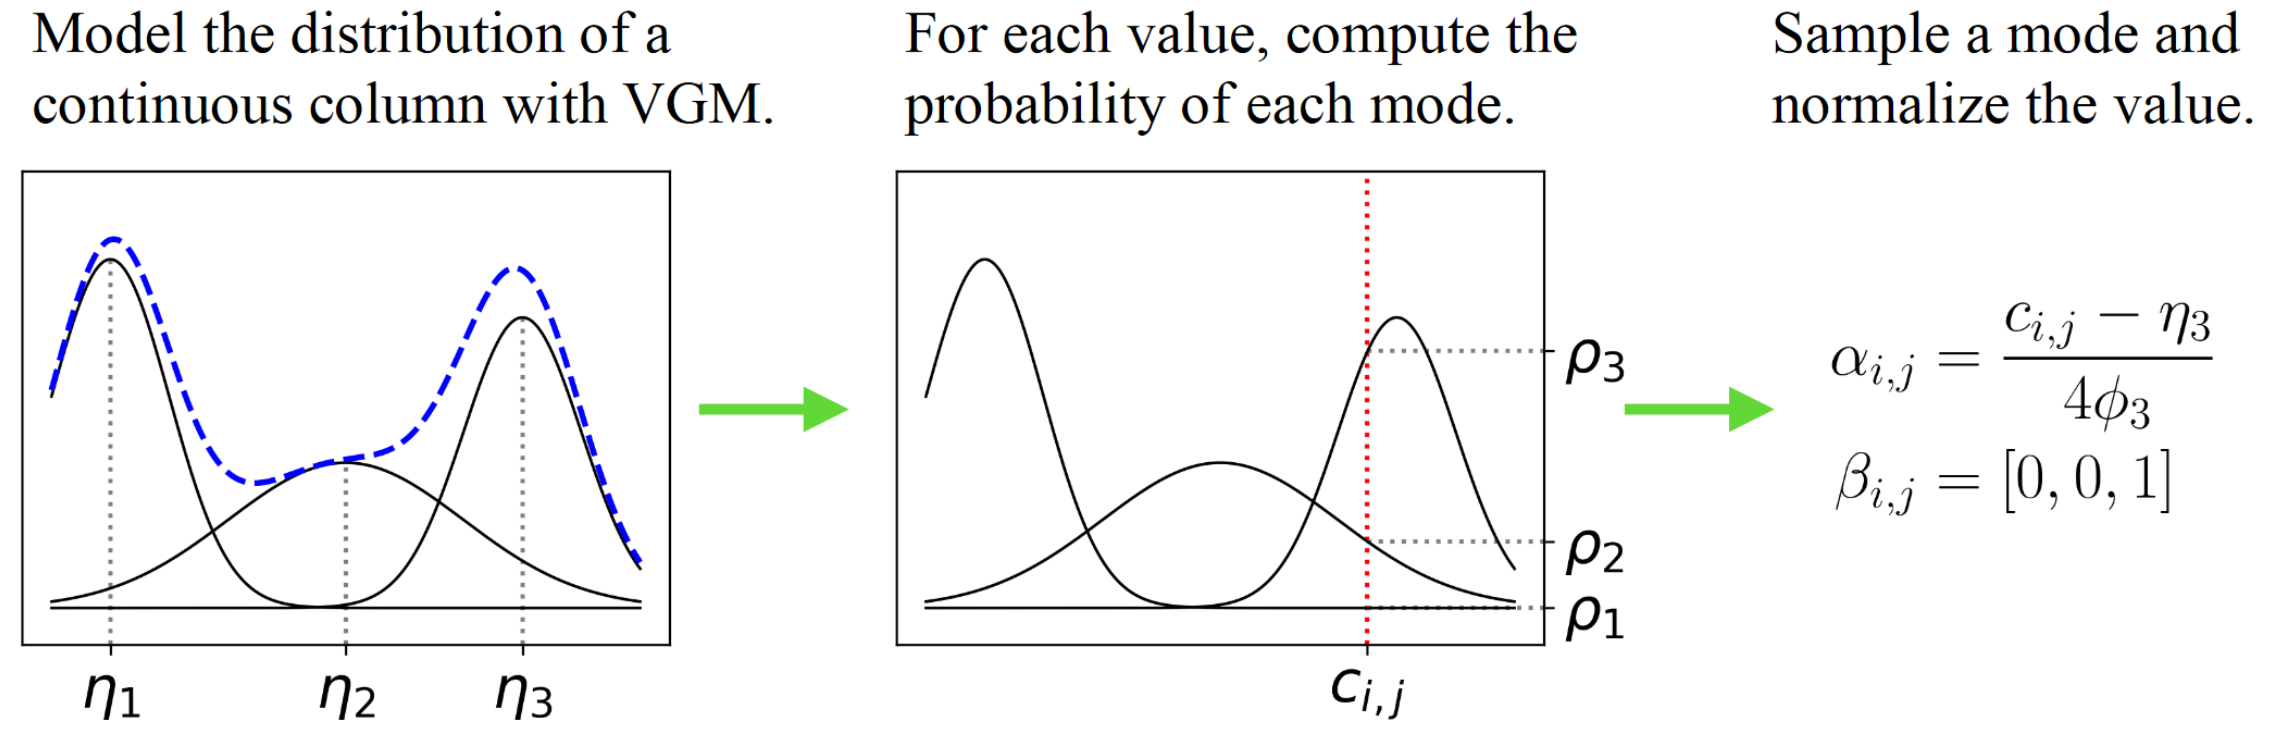
\includegraphics[width=0.5\textwidth]{images/mode-normalization.png}
    \caption{An example of mode-specific normalization [TODO: COPYRIGHT?] \cite[Figure 1, p. 4]{xu2019ModelingTabularData}}
    \label{fig:mode-specific-normalization}
  \end{figure}


Another approach to standardize the range of a column between 0 and 1 is a Quantile-Transformation, a non-linear transformation \cite{scikit-learnPreprocessingData, kotelnikov2022TabDDPMModellingTabular}.
The Quantile-transformation allows to map all values of a random variable into an desired output distribution, such as the uniform or normal distribution, 
using the quantile function on the inverse cumulative distribution of the random variable. This transformation preserves the rank order of the values but distorts correlations and distances within and across features \cite{scikit-learnPreprocessingData}.

\subsection{Synthetic Tabular Data Generation}

Generative models have recently received a lot of attention, thanks to their impressive results generating a variety of data formats, 
such as images \cite{ho2020DenoisingDiffusionProbabilistic, dhariwal2021DiffusionModelsBeat, rombach2022HighResolutionImageSynthesis}, videos \cite{ho2022VideoDiffusionModels, Gen1Runway}, text \cite{radfordImprovingLanguageUnderstanding, 2022ChatGPTOptimizingLanguage} or music \cite{agostinelli2023MusicLMGeneratingMusic, martirosRiffusion}.

While synthetic data generation can be applied to various types of data, generating synthetic tabular data is a challenging task due to the complexity of the underlying joint distributions between variables.
This work adapts the formal definition of the tabular data generation adapted from \cite[p. 2]{xu2019ModelingTabularData}:

\begin{displayquote}
    A data synthesizer $G$ is trained on a table $T$ and then used to generate a synthetic table $T_{syn}$. % Vllt die definition einer tabelle nach oben packen und von oben übernehmen?
    $T$ consists of $N_c$ continuos columns ${C_1, ..., C_{N_c}}$ and $N_d$ categorical columns (or a discrete representation of it) ${D_1, ..., D_{N_d}}$
    Each column is considered to be a random variable and follows an unknown joint distribution $\mathbb{P}(C_{1:N_c},D_{1:N_d})$.
    One row $r_j=\{c_{1,j}, ...,c_{N_c,j}, d_{1,j}, ...,d_{N_d,j}\}$, $j \in\{1, ..., n\}$, is one observation from the joint distribution.
    $T$ is partitioned into a training set $T_{train}$ and test set $T_{test}$. 
    The synthesizer $G$ is trained on $T_{train}$ and afterwards used to sample independently individual rows to create $T_{syn}$.
\end{displayquote}

During the generation of synthetic tabular data there are two competing objectives, high data utility and low disclosure risk.
Data utility is concerned with how well the synthetic data accurately reflects the real data in terms of its underlying patterns and relationships.
Low disclosure risk on the other hand is concerned with the preservation of privacy and confidentiality of the information in the real training dataset $T_{train}$ \cite{little2021GenerativeAdversarialNetworksa}. 

Tabular data synthesis approaches can be summarized into Process and data driven methods \cite{goncalves2020GenerationEvaluationSynthetic}.
Process driven models focus on simulating real world processes and gather data during that simulation to create the synthetic dataset \cite{kowalczyk2022TaxonomyUseSynthetic}.
On the other hand, data driven approaches aim to generate synthetic data based on already existing real-world dataset \cite{kowalczyk2022TaxonomyUseSynthetic}.
This can be achieved by augmenting the existing dataset, \ie applying transformations to the existing datapoints to generate new datapoints \cite{kowalczyk2022TaxonomyUseSynthetic}s.
Another technique to generate synthetic data is to simply sample from the individual feature distributions of a dataset to generate new synthetic data \cite{kowalczyk2022TaxonomyUseSynthetic}.
Lastly, machine learning and deep learning algorithms can be used to learn the underlying joint distributions of the real data to generate new synthetic data \cite{kowalczyk2022TaxonomyUseSynthetic}. 

%challanges
The synthesis of tabular data is, compared to other data types, especially challenging due to its heterogeneity, potential weak correlations among feature and dependency on preprocessing \cite{borisov2022DeepNeuralNetworks, yoon2020VIMEExtendingSuccess, gorishniy2022EmbeddingsNumericalFeatures}.
To create a realistic synthetic dataset interdependencies that may exists between variables must be captured and 
it is possible that the \gls{model} overfits on the training data and generalizes relationships between features that are only present in training but not test data \cite{lederrey2022DATGANIntegratingExperta}
In addition to that, tabular data columns can follow complex distributions, that make the synthesization challenging.
\cite{zhao2022CTABGANEnhancingTabular} identifies the following four properties of tabular data:

\begin{enumerate}
    \item Single Gaussian variables: Data where its distribution follows a gaussian distribution \cite{zhao2022CTABGANEnhancingTabular}.
    \item Mixed data type variables: A single column can contain a mix of continuos and categorical values. 
    For instance, a "loan" column could hold information about the size of an individuals loan.
    The values in this column are mostly positive float values but can also take the value "-1" which indicates, that this person did not get approach for a loan.
    Such a special categorical value in an otherwise numerical column need to be considered when working with this column \cite{zhao2022CTABGANEnhancingTabular}.
    \item Long tail distributions: In real world data (especially sales data), it can occur that most occur "near the initial value of a distribution and rare cases towards the end" \cite[p. 3]{zhao2022CTABGANEnhancingTabular}.
    This results in a tail-like distribution.
    \item Skewed multi-mode continuous variables: Complex numerical distributions do not necessarily follow a single gaussian distributions.
    It is possible for their distribution to consist of multiple unknown distributions that are potential skewed as well. 
    Their conjunction as a whole makes up the complex distribution \cite{zhao2022CTABGANEnhancingTabular}.
\end{enumerate}

A successful tabular data generator should be able to recreate such properties of real data in their synthetic data counterpart.



%-------------------------------------------------------------------------
\section{Deep Learning Architectures}
\label{ch:preliminaries-deepLearningArchitectures}

Deep learning has rapidly become a dominant force in artificial intelligence, revolutionizing various fields including computer vision, natural language processing, and data generation. 
Complex architectures made up of many layers of artificial neural networks are used to build deep learning models.
These architectures have enabled the creation of highly accurate and efficient models that are capable of processing vast amounts of data. 
In recent years, the development of new deep learning architectures has been a key area of research, leading to the creation of powerful models.
This section will start with a high-level introduction into the most important architectural building blocks of a neural network.
Afterwards the most important deep learning \gls{model} architectures for generating data are presented.

\subsection{Neural Networks}
\label{ch:preliminaries-deepLearningArchitectures-neuralNetworks}

The most basic neural network is called a perceptron \cite{rosenblatt1958PerceptronProbabilisticModel}.
It consists of a single input layer that is connected to an output node.
Each input node is connected with the output node via weight edges.
For all inputs, the input value is multiplied with each respective weight.
The sum of all input-weight multiplication serves as the input to an activation function, which is different depending of the task at hand.
The output is the prediction of the perceptron which is compared to the actual result, the label, and an error is calculated.
This error is used later on to update the weights of the individual nodes via backpropagation \cite{aggarwal2018NeuralNetworksDeep}.
The output of one node can also serve as the input to another node, so multiple layers of nodes are created.
This is refereed to as a \gls{mlp} or feed-forward neural network, 
because the information flows forward from input through the multiple layers in the middle (also called hidden layers) to the output \cite{aggarwal2018NeuralNetworksDeep, Goodfellow-et-al-2016}.
An \gls{mlp} tries to approximate some function $f*$ by defining a mapping $y=f(x;\theta)$ by learning the values of the parameters $\theta$ (\ie the weights) that best approximate $f*$ \cite{Goodfellow-et-al-2016}.
A simple \gls{mlp} is already able to learn any "reasonable" function, which is why they are also considered to be universal function approximators \cite{aggarwal2018NeuralNetworksDeep, hornik1989MultilayerFeedforwardNetworks}.

Convolutional networks, or \glspl{cnn} \cite{lecun1998GradientbasedLearningApplied}, are a specialized type of neural network.
As their name indicate, they perform convolutions on the data.
A convolution can be defined as "a dot-product operation between a grid-structured set of weights and similar grid-structured inputs drawn from
different spatial localities in the input volume" \cite[p. 316]{aggarwal2018NeuralNetworksDeep}.
They perform exceptionally well on data with a grid-like topology, with strong spatial dependencies, such as image or time-series data \cite{aggarwal2018NeuralNetworksDeep, Goodfellow-et-al-2016}.
In a typical convolutional network, a layer starts by performing multiple convolution operations in parallel on the data.
The linear activations that are produced by the convolutions are send through a nonlinear activation function (usually a \gls{relu}).
Lastly, a pooling function is applied to the output of the activation function.
A pooling function reduces the spatial size of the created feature maps while retaining their essential features \cite{Goodfellow-et-al-2016, aggarwal2018NeuralNetworksDeep}.
It can be described as a type of "summary statistic of the nearby outputs" \cite[p. 335]{Goodfellow-et-al-2016}.
Pooling allows the features extracted by the \gls{cnn} to be less sensitive to changes in the position of the input data.
This property is known as translation invariance and is one of the reasons why \glspl{cnn} perform so well with data formats that have local spatial dependencies \cite{Goodfellow-et-al-2016, aggarwal2018NeuralNetworksDeep}.

In feed-forward neural networks information flows forward through the network from input to output node, hence, there are no internal connections that allow
the output of the model to be fed back into the network as inputs \cite{aggarwal2018NeuralNetworksDeep, Goodfellow-et-al-2016}.
When such connections are added to the network architecture, the resulting models are referred to as \glspl{rnn} \cite{rumelhart1986LearningRepresentationsBackpropagating}.
\Glspl{rnn} are design to process sequential data, like sentences or time-series data, where the size of the sequence does not have to be fixed.
In \glspl{cnn} the learned parameters are shared by using the same convolution kernel on each subset of neighbouring input data at each time step. 
As a result, a succession of output values is produced, each of which is dependent on a few close input values. 
On the other hand, \glspl{rnn} share parameters differently since each output value depends on the predecessor output of it it. 
This enables parameter sharing via a deep computational graph by enabling the same update algorithm to be applied to all outputs.
When processing a sequence, \eg a sentence, an \gls{rnn} receives one datapoint,\eg a word, at each timestep.
The network itself has a so called hidden-state that is kept throughout all timesteps and changes with each timestep.
This however means, that the output $y_3$ of the input at $x_{t=3}$ depends on the hidden-states $h_0$ through $h_3$ and input $x_0$ through $x_3$.
As a result, the computational graph where the backpropagation is performed on increases as well \cite{aggarwal2018NeuralNetworksDeep}.
A large computation graph introduces new practical issues, such as an increased computation time and during the training useful information might not be propagated from output to the end of the model,
due to the makes the vanishing and exploding gradient phenomenon \cite{aggarwal2018NeuralNetworksDeep}.
To address these issue, further improvements to the architecture have been made, such as \glspl{lstm} \cite{hochreiter1997LongShortTermMemory} or \glspl{gru} \cite{cho2014PropertiesNeuralMachine}.

Over time, additional architectural design choices have been discovered that have led to further improvements and solved other issues that emerged during the development of neural networks.
One such design is the ResNet \cite{he2016DeepResidualLearning} which introduced residual connections between layers \cite{he2016DeepResidualLearning, aggarwal2018NeuralNetworksDeep}.
The connections, also called skip connections, allowed that information can be copied over layers and allows the backpropagated gradient information to skip certain layers, if necessary \cite{he2016DeepResidualLearning, aggarwal2018NeuralNetworksDeep}.
This is achieved by adding the output of one layer directly to the output of a later layer, bypassing one or more intermediate layers.
During backpropagation of the gradient, a very small gradient can flow this way more easily back through the network,  alleviating the vanishing gradient problem and enabling better learning capabilities \cite{he2016DeepResidualLearning, aggarwal2018NeuralNetworksDeep}.
The decision of which layers to skip is learned by the model itself during the training through the backpropagation algorithm \cite{he2016DeepResidualLearning, aggarwal2018NeuralNetworksDeep}.

Lastly, inspired by the human cognitive capabilities to focus on specific parts of an input, attention mechanisms have been introduced \cite{niu2021ReviewAttentionMechanism, aggarwal2018NeuralNetworksDeep}.
The implementation of attention in neural networks tries to address the problem of information overload, and is supposed to enable the network to allocate their resources \cite{niu2021ReviewAttentionMechanism}.
An attention mechanism has been successfully applied to various tasks in different domains, such as computer vision or natural language processing \cite{niu2021ReviewAttentionMechanism}.
The architectural realization of attention is realized differently, depending on the task at hand \cite{aggarwal2018NeuralNetworksDeep}.
The attention mechanism in computer vision involves weighting different regions of the image based on their relevance to the task \cite{aggarwal2018NeuralNetworksDeep}. 
This can be achieved through techniques such as spatial attention, channel attention or temporal attention \cite{guo2022AttentionMechanismsComputer}.
In natural language processing attention mechanism try to improve to capture the meaning of a sentence \cite{niu2021ReviewAttentionMechanism}. 
For instance, this has been achieved through the introduction of a context vector in an \gls{rnn} encoder-decoder \cite{DBLP:journals/corr/BahdanauCB14} or through self-attention \cite{vaswani2017AttentionAllYou} (see \autoref{ch:preliminaries-generativeAlgorithms-transformers} for a detailed explanation on self-attention).


\section{Generative Algorithms}
\label{ch:preliminaries-generativeAlgorithms}

\subsection{Autoencoders}
\label{ch:preliminaries-generativeAlgorithms-variationalAutoencoders}

from \cite{kingma2013AutoEncodingVariationalBayes}

Figure 1 from \cite{razghandi2022VariationalAutoencoderGenerativea}

% what are autoencoders
encoder transforms input into latent space which is reconstructed by decoder \cite{razghandi2022VariationalAutoencoderGenerativea}
--> suffer from "lack of regularity in latent space \cite{razghandi2022VariationalAutoencoderGenerativea}

% what are variational autoencoders
use the KL divergence and encode a gaussian distribution in latent space \cite{razghandi2022VariationalAutoencoderGenerativea}
% how do they work
% mathematical formulation
% Advantages / Problems / Challenges


\subsection{Generative Adversarial Networks}
\label{ch:preliminaries-generativeAlgorithms-generativeAdversarialNetworks}

% what are GAN's
\cite{goodfellow2020GenerativeAdversarialNetworks}
- have been used very sucessfully in many different domains \cite{li2022TTSGANTransformerbasedTimeSeries}
 

% how do they work
\cite{zhao2022CTABGANEnhancingTabular}:
- trained via a zero-sum min-max game 
- the discriminator tries to maximize the objective, while the generator tries to minimize it.
- mentor (D) providing feedback to a student (G) on the quality of his work


\cite{li2022TTSGANTransformerbasedTimeSeries}
- 2 NN (gen and dis)
- gen inp: rand vec of specified dimension; gen out: same dimension, as similar to real training data
- dis: binary classifier, distiguish real and generated data
--> play zero sum game against each other
--> trz to each nash equilibrium

% what improvements have been done to GAN's
- gans struggled with generating discrete variables \cite{torfi2020CorGANCorrelationCapturingConvolutionala}
- State of the art Gan approaches only focused on continouse and categorical types, overlooking mixed data types \cite{zhao2022CTABGANEnhancingTabular}

- conditional GAN \cite{mirza2014ConditionalGenerativeAdversarial}


% mathematical formulation
% Advantages / Problems / Challenges (Mode Collapse, etc.)
- remarkable performance generating syntehtic images and time series data \cite{mckeever2020SynthesisingTabularDatasets}
- struggle with mode collapse --> generate same sample \cite{torfi2020CorGANCorrelationCapturingConvolutionala}
- wasserstein loss helps against mode collapse \cite{frogner2015LearningWassersteinLoss} \cite{arjovsky2017WassersteinGenerativeAdversarial} and has been implemented in many gans (e.g. \cite{zhao2022CTABGANEnhancingTabular})
- gradient penalty \cite{gulrajani2017ImprovedTrainingWasserstein}


\subsection{Transformers}
\label{ch:preliminaries-generativeAlgorithms-transformers}
relies on multiple self-attention layers, surpasses other network architectures and shows properties of universal computation engine \cite{li2022TTSGANTransformerbasedTimeSeries}

have been very successfull on textual and visual data (//siehe quellen im paper) \cite{borisov2022DeepNeuralNetworks} and also been applied to tabular data \cite{padhi2021TabularTransformersModeling} \cite{gorishniy2022EmbeddingsNumericalFeatures}



% What are transformers
% How do they work
% In what context are they used (usually not for data synthesis)
% Advantages / Problems / Challenges

- TabNet is one of the first transformer-based models for tabular data \cite{borisov2022DeepNeuralNetworks}
- padhi2021TabularTransformersModeling

\subsection{Diffusion Probabilistic Models}
\label{ch:preliminaries-generativeAlgorithms-diffusionProbabilisticModels}

% What are diffusion probabilistic models
first paper \cite{sohl-dickstein2015DeepUnsupervisedLearning}
first famouse paper \cite{ho2020DenoisingDiffusionProbabilistic}
improvements> \cite{nichol2021ImprovedDenoisingDiffusion}
follow up: \cite{dhariwal2021DiffusionModelsBeat}

\cite{ho2022ClassifierFreeDiffusionGuidance}

\cite{rombach2022HighResolutionImageSynthesis}

% mathematical formulation
% How do they work
% In what context are they used (usually image synthesis)
% Advantages / Problems / Challenges


% for tabular data
\cite{zheng2022DiffusionModelsMissing} for missing data

\cite{kotelnikov2022TabDDPMModellingTabular} tabddpm
\cite{hoogeboom2021ArgmaxFlowsMultinomial} multinomial diffusion


\subsection{Diffusion Probabilistic Models for Tabular Data}
\label{ch:preliminaries-generativeAlgorithms-diffusionProbabilisticModelsTabularData}

% How can Diffusion Probabilistic Models be used for tabular data
% Challenges of using Diffusion Probabilistic Models for tabular data (mixed data types --> different noising process, etc.)


%-------------------------------------------------------------------------
\section{Evaluation of Synthetic Tabular Data}
\label{ch:preliminaries-evaluationOfSyntheticTabularData}

- there is no universal metric for data synthesis \cite{hernandez2022SyntheticDataGeneration}
- utility and information disclosure metric dimensions \cite{goncalves2020GenerationEvaluationSynthetic}
- structural similarity \cite{elemam2020SevenWaysEvaluate}

\subsection{Statistical Evaluation}
\label{ch:preliminaries-evaluationOfSyntheticTabularData-statisticalEvaluation}

\subsection{Machine Learning Efficiency}
\label{ch:preliminaries-evaluationOfSyntheticTabularData-machineLearningEfficiency}

\subsection{Privacy Evaluation}
\label{ch:preliminaries-evaluationOfSyntheticTabularData-privacyEvaluation}

\subsection{Additional Evaluation Methods}
\label{ch:preliminaries-evaluationOfSyntheticTabularData-otherMetrics}

% Bias and stability
% Domain Expertise

\subsection{Similarity Score}
\label{ch:preliminaries-evaluationOfSyntheticTabularData-similarityScore}
% https://www.researchgate.net/publication/344227988_On_the_Generation_and_Evaluation_of_Tabular_Data_using_GANs

% TOREAD: https://www.researchgate.net/publication/361949372_TabSynDex_A_Universal_Metric_for_Robust_Evaluation_of_Synthetic_Tabular_Data

%-------------------------------------------------------------------------




